\chapter{結言}
\thispagestyle{myheadings}

\section{まとめ}
本研究では,ベッド型の下肢リハビリ装置を拡張する没入型歩行感覚提示システムを提案し,大学生の被験者に対して提案システムの印象に関するアンケート調査を行った.SD法を用いたアンケートの結果より,提案システムに対して肯定的な意見が確認され,リハビリへのモチベーション向上が期待される.今後の課題として,「作動音がうるさい」という問題点を解決するために,被験者にヘッドフォンを着用し,生活音を利用した没入感の向上が検討される.また,「歩いている距離が短い」という問題を解決するために,被験者の足の長さに合わせたCGキャラクタの移動距離の変更の実装も考えられる.
\section{今後の課題}
本節では,提案システムを使用した評価実験に基づいた今後の課題について述べる.
本研究における今後の課題として,提案システム内での音の考慮,複数人での提案システムの使用による相乗効果の検討,応用としてKinectとHMDを使用した歩行感覚提示システムの応用などが挙げられる.以下に各課題について述べる.
\subsection{音の考慮}
「寂しい」という意見やベッド型の下肢リハビリ装置の作動音がうるさいという意見があげられたので,ヘッドフォンを着用し,生活音も出力するシステムへの変更も検討される.これにより臨場感が高まり,没入感の向上が期待できる.

\subsection{歩幅の変更}
「歩いている距離が短い」という意見から,被験者の歩幅に合ったキャラクタの移動距離の変更を実装する必要が検討される.性差や各年代の歩幅を調べ性別や年齢を入力することでキャラクタの移動を変更するシステムが考えられる.

\subsection{複数人での使用による相乗効果の検討}
実験環境で使用したUnityのオンラインシステムを使用し,複数人でコミュニケーションを取りながらリハビリを行えるシステムも考えられる.
これにより,寂しさや単調さを解消が期待される.

\subsection{KinectとHMDを使用したリハビリ}
ヘルス・リテラシーの向上を目指し,「23区VRウォーキング」が開発されている.図\ref{fig:VR1}に示す,仮想空間をKinectを使用してユーザの動作を検出し,図\ref{fig:KHR-1}--\ref{fig:KHR-2}に示す足踏みの動作によってキャラクタが移動するコンテンツとなっている.そこで今回開発したHMDを使用した歩行感覚提示装置とKinectを使用し,「23区VRウォーキング」よりも没入感の高いコンテンツに応用可能と考えられる.

\begin{figure}[tbp]
	\centering
			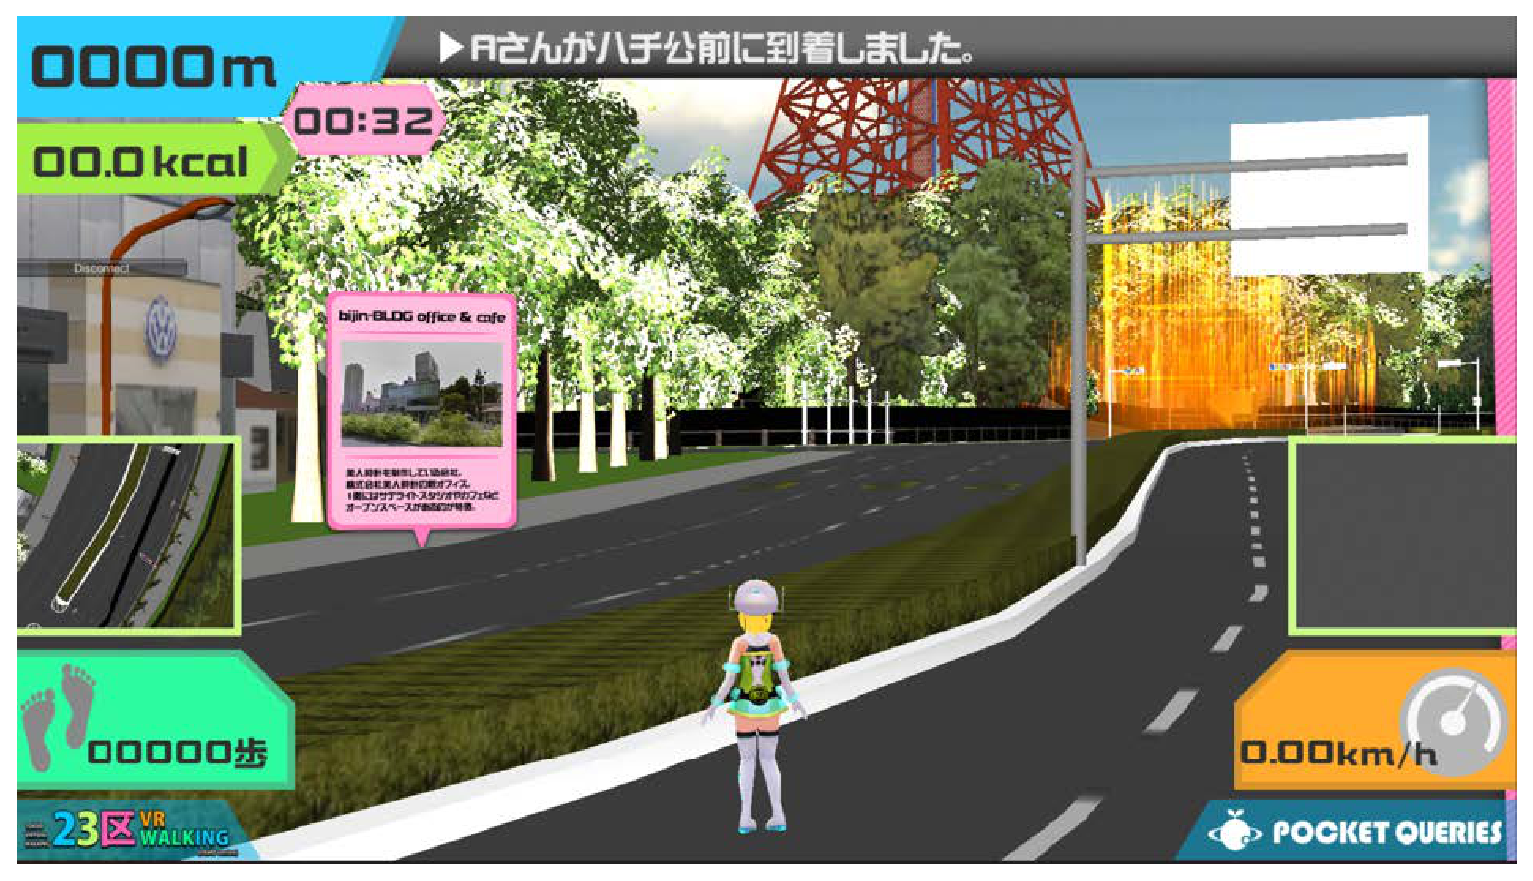
\includegraphics[width=0.9\textwidth]{chap4-figure/VR1.eps}
	\caption{関連コンテンツ(文献\cite{VR}より引用)}
	\label{fig:VR1}
\end{figure}

\begin{figure}[tbp]
	\centering
			\includegraphics[width=0.9\textwidth]{chap4-figure/kine_ocu_1.eps}
	\caption{KinectとHMDを使用した足踏みのリハビリの例(横からの図)}
	\label{fig:KHR-1}
\end{figure}
\begin{figure}[tbp]
	\centering
			\includegraphics[width=0.9\textwidth]{chap4-figure/kine_ocu_2.eps}
	\caption{KinectとHMDを使用した足踏みのリハビリの例(正面からの図)}
	\label{fig:KHR-2}
\end{figure}


% Local Variables: 
% mode: japanese-LaTeX
% TeX-master: "root"
% End: 
